\documentclass{article}
\def \insidegridcolor {gray}
\def \cellwidth {1.5}
\def \cellheight {\cellwidth*1.5}
% D--H--C
% |     |
% I  X  J
% |     |
% E--G--F
% |     |
% A-----B
% point A is at (0,0)
\def \pointA {(0+\x*\cellwidth,0+\y*\cellheight)}
% point B is at (1,0)
\def \pointB {(\cellwidth+\x*\cellwidth,0+\y*\cellheight)}
% point C is at (1,1.5)
\def \pointC {(\cellwidth+\x*\cellwidth,\cellheight+\y*\cellheight)}
% point D is at (0,1.5)
\def \pointD {(0+\x*\cellwidth,\cellheight+\y*\cellheight)}
% point E is at (0,0.5)
\def \pointE {(0+\x*\cellwidth,\cellheight/3+\y*\cellheight)}
% point F is at (1,0.5)
\def \pointF {(\cellwidth+\x*\cellwidth,\cellheight/3+\y*\cellheight)}
% point G is at (0.5,0.5)
\def \pointG {(\cellwidth/2+\x*\cellwidth,\cellheight/3+\y*\cellheight)}
% point H is at (1.5,1.5)
\def \pointH {(\cellwidth/2+\x*\cellwidth,\cellheight+\y*\cellheight)}
% point I is at (0,1.5)
\def \pointI {(0+\x*\cellwidth,\cellheight/3*2+\y*\cellheight)}
% point J is at (1,1)
\def \pointJ {(\cellwidth+\x*\cellwidth,\cellheight/3*2+\y*\cellheight)}

\usepackage{tikz}
\usepackage[margin=0.5in]{geometry}
\begin{document}
\pagenumbering{gobble}
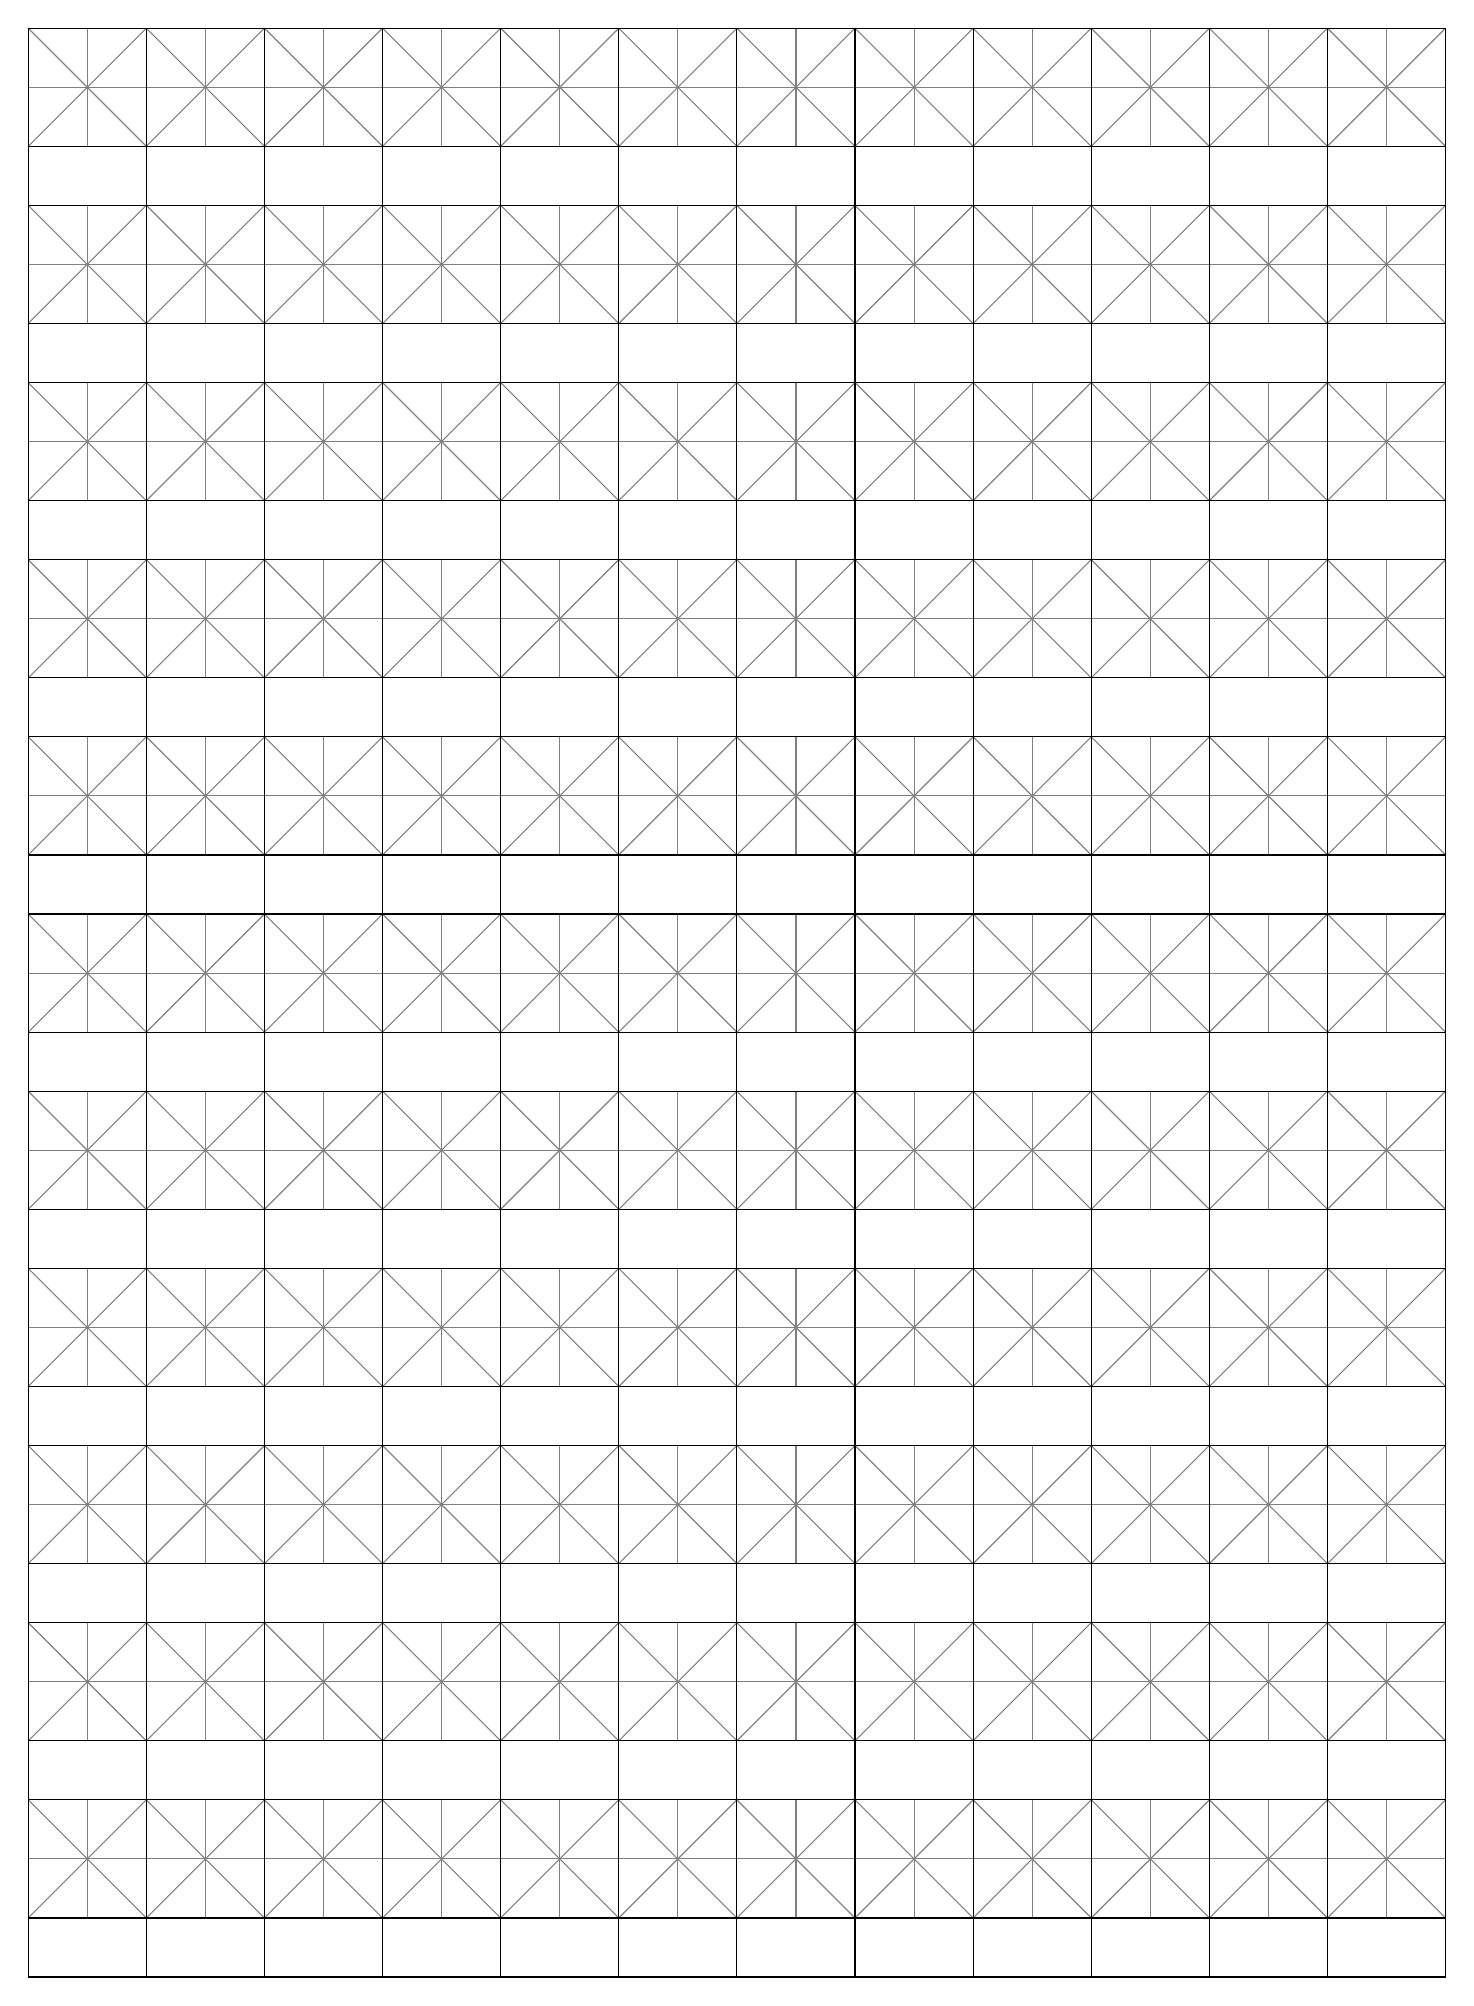
\begin{tikzpicture}
\foreach \y in {0,...,10}
\foreach \x in {0,...,11}
{
% Draw the X
\draw[\insidegridcolor] \pointE -- \pointC;
\draw[\insidegridcolor] \pointF -- \pointD;
% Draw the +
\draw[\insidegridcolor] \pointG -- \pointH;
\draw[\insidegridcolor] \pointI -- \pointJ;
% Draw the outside box
\draw \pointA -- \pointB -- \pointC -- \pointD -- \pointA;
% Draw the line separating the character box from the pinyin box
\draw \pointE -- \pointF;
}
\end{tikzpicture}
\end{document}